\documentclass[11pt,a4paper]{report}
\usepackage[textwidth=37em,vmargin=30mm]{geometry}
\usepackage{calc,xunicode,amsmath,amssymb,paralist,enumitem,tabu,booktabs,datetime2,xeCJK,xeCJKfntef,listings}
\usepackage{tocloft,fancyhdr,tcolorbox,xcolor,graphicx,eso-pic,xltxtra,xelatexemoji}

\newcommand{\envyear}[0]{2025}
\newcommand{\envdatestr}[0]{2025-08-25}
\newcommand{\envfinaldir}[0]{webdb/2025/20250825/final}

\usepackage[hidelinks]{hyperref}
\hypersetup{
    colorlinks=false,
    pdfpagemode=FullScreen,
    pdftitle={Web Digest - \envdatestr}
}

\setlength{\cftbeforechapskip}{10pt}
\renewcommand{\cftchapfont}{\rmfamily\bfseries\large\raggedright}
\setlength{\cftbeforesecskip}{2pt}
\renewcommand{\cftsecfont}{\sffamily\small\raggedright}

\setdefaultleftmargin{2em}{2em}{1em}{1em}{1em}{1em}

\usepackage{xeCJK,xeCJKfntef}
\xeCJKsetup{PunctStyle=plain,RubberPunctSkip=false,CJKglue=\strut\hskip 0pt plus 0.1em minus 0.05em,CJKecglue=\strut\hskip 0.22em plus 0.2em}
\XeTeXlinebreaklocale "zh"
\XeTeXlinebreakskip = 0pt


\setmainfont{Brygada 1918}
\setromanfont{Brygada 1918}
\setsansfont{IBM Plex Sans}
\setmonofont{JetBrains Mono NL}
\setCJKmainfont{Noto Serif CJK SC}
\setCJKromanfont{Noto Serif CJK SC}
\setCJKsansfont{Noto Sans CJK SC}
\setCJKmonofont{Noto Sans CJK SC}

\setlength{\parindent}{0pt}
\setlength{\parskip}{8pt}
\linespread{1.15}

\lstset{
	basicstyle=\ttfamily\footnotesize,
	numbersep=5pt,
	backgroundcolor=\color{black!5},
	showspaces=false,
	showstringspaces=false,
	showtabs=false,
	tabsize=2,
	captionpos=b,
	breaklines=true,
	breakatwhitespace=true,
	breakautoindent=true,
	linewidth=\textwidth
}






\newcommand{\coverpic}[2]{
    % argv: itemurl, authorname
    Cover photo by #2~~(\href{#1}{#1})
}
\newcommand{\makeheader}[0]{
    \begin{titlepage}
        % \newgeometry{hmargin=15mm,tmargin=21mm,bmargin=12mm}
        \begin{center}
            
            \rmfamily\scshape
            \fontspec{BaskervilleF}
            \fontspec{Old Standard}
            \fontsize{59pt}{70pt}\selectfont
            WEB\hfill DIGEST
            
            \vfill
            % \vskip 30pt
            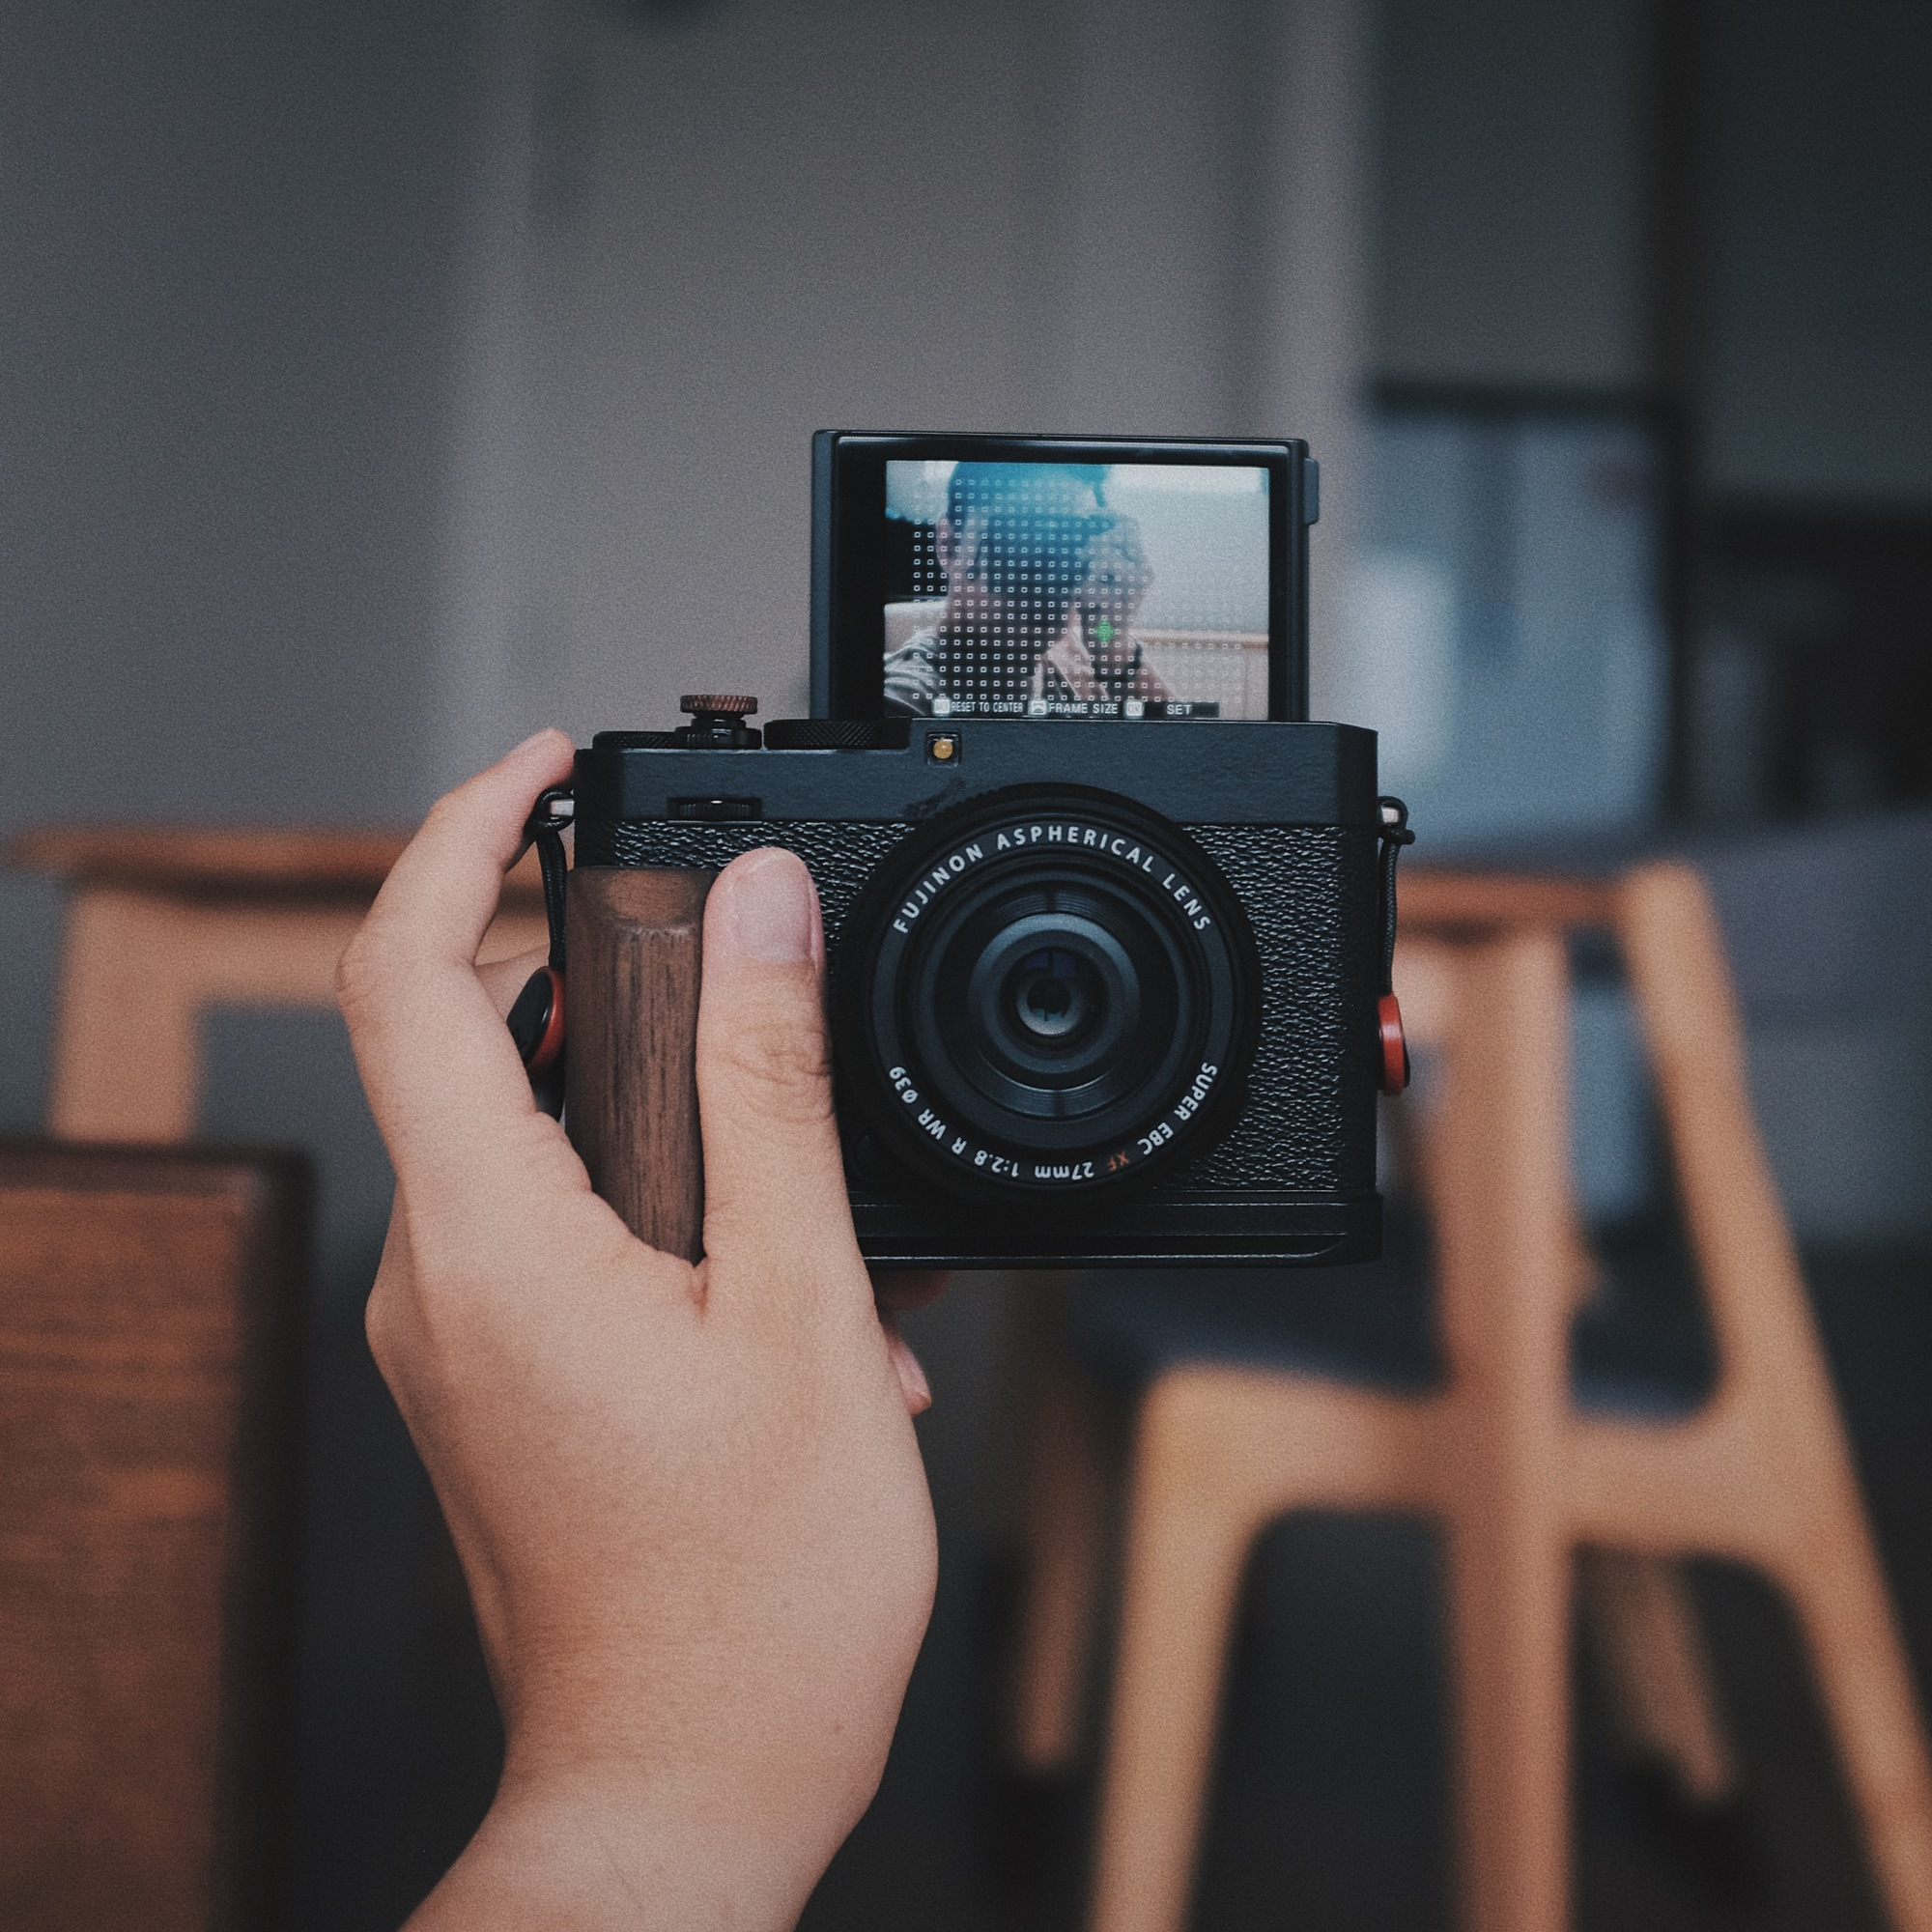
\includegraphics[width=\linewidth]{\envfinaldir/coverpic-prod.jpg}\par
            % \vskip 30pt
            \vfill

            \normalsize\rmfamily\scshape
            \copyright{} The Web Digest Project \hfill\large \envdatestr
        \end{center}
    \end{titlepage}
    % \restoregeometry
}
\newcommand{\simplehref}[1]{%
    \textcolor{blue!80!green}{\href{#1}{#1}}%
}
\renewcommand{\contentsname}{\center\Huge\sffamily\bfseries Contents\par\vskip 20pt}
\newcounter{ipartcounter}
\setcounter{ipartcounter}{0}
\newcommand{\ipart}[1]{
    % \vskip 20pt
    \clearpage
    \stepcounter{ipartcounter}
    \phantomsection
    \addcontentsline{toc}{chapter}{#1}
    % \begin{center}
    %     \Huge
    %     \sffamily\bfseries
    %     #1
    % \end{center}
    % \vskip 20pt plus 7pt
}
\newcounter{ichaptercounter}
\setcounter{ichaptercounter}{0}
\newcommand{\ichapter}[1]{
    % \vskip 20pt
    \clearpage
    \stepcounter{ichaptercounter}
    \phantomsection
    \addcontentsline{toc}{section}{\numberline{\arabic{ichaptercounter}}#1}
    \begin{center}
        \Huge
        \sffamily\bfseries
        #1
    \end{center}
    \vskip 20pt plus 7pt
}
\newcommand{\entrytitlefont}[1]{\subsection*{\raggedright\Large\sffamily\bfseries#1}}
\newcommand{\entryitemGeneric}[2]{
    % argv: title, url
    \parbox{\linewidth}{
        \entrytitlefont{#1}\par\vskip 5pt
        \footnotesize\ttfamily\mdseries
        \simplehref{#2}
    }\vskip 11pt plus 11pt minus 1pt
}
\newcommand{\entryitemGithub}[3]{
    % argv: title, url, desc
    \parbox{\linewidth}{
        \entrytitlefont{#1}\par\vskip 5pt
        \footnotesize\ttfamily\mdseries
        \simplehref{#2}\par\vskip 5pt
        \small\rmfamily\mdseries#3
    }\vskip 11pt plus 11pt minus 1pt
}
\newcommand{\entryitemAp}[3]{
    % argv: title, url, desc
    \parbox{\linewidth}{
        \entrytitlefont{#1}\par\vskip 5pt
        \footnotesize\ttfamily\mdseries
        \simplehref{#2}\par\vskip 5pt
        \small\rmfamily\mdseries#3
    }\vskip 11pt plus 11pt minus 1pt
}
\newcommand{\entryitemHackernews}[3]{
    % argv: title, hnurl, rawurl
    % \parbox{\linewidth}{
    %     \entrytitlefont{#1}\par\vskip 5pt
    %     \footnotesize\ttfamily\mdseries
    %     \simplehref{#3}\par
    %     \textcolor{black!50}{\href{#2}{#2}}
    % }\vskip 11pt plus 11pt minus 1pt
    \begin{minipage}{\linewidth}
            \entrytitlefont{#1}\par\vskip 5pt
            \footnotesize\ttfamily\mdseries
            \simplehref{#3}\par
            \textcolor{black!50}{\href{#2}{#2}}
    \end{minipage}\par\vskip 11pt plus 11pt minus 1pt
}







\begin{document}

\makeheader

\tableofcontents\clearpage




\ipart{Developers}
\ichapter{Hacker News}
\entryitemTwoLinks{Starship's Tenth Flight Test}{https://news.ycombinator.com/item?id=45007907}{https://www.spacex.com/launches/starship-flight-10}

\entryitemTwoLinks{Everything I know about good API design}{https://news.ycombinator.com/item?id=45006801}{https://www.seangoedecke.com/good-api-design/}

\entryitemTwoLinks{Paracetamol disrupts early embryogenesis by cell cycle inhibition}{https://news.ycombinator.com/item?id=45006296}{https://academic.oup.com/humrep/advance-article/doi/10.1093/humrep/deaf116/8234396}

\entryitemTwoLinks{Is 4chan the perfect Pirate Bay poster child to justify wider UK site-blocking?}{https://news.ycombinator.com/item?id=45005545}{https://torrentfreak.com/uk-govt-finds-ideal-pirate-bay-poster-boy-to-sell-blocking-of-non-pirate-sites-250824/}

\entryitemTwoLinks{Comet AI browser can get prompt injected from any site, drain your bank account}{https://news.ycombinator.com/item?id=45004846}{https://twitter.com/zack\_overflow/status/1959308058200551721}

\entryitemTwoLinks{Making games in Go: 3 months without LLMs vs. 3 days with LLMs}{https://news.ycombinator.com/item?id=45004728}{https://marianogappa.github.io/software/2025/08/24/i-made-two-card-games-in-go/}

\entryitemTwoLinks{US attack on renewables will lead to power crunch that spikes electricity prices}{https://news.ycombinator.com/item?id=45004466}{https://www.cnbc.com/2025/08/24/solar-wind-renewable-trump-tariff-utility-tax-credit-itc-ptc-obbb-electricity-price.html}

\entryitemTwoLinks{ICE uses celebrity loophole to hide deportation flights}{https://news.ycombinator.com/item?id=45003819}{https://jacobin.com/2025/08/ice-uses-celebrities-loophole-to-hide-deportation-flights/}

\entryitemTwoLinks{Dynamically patch a Python function's source code at runtime}{https://news.ycombinator.com/item?id=45003750}{https://ericmjl.github.io/blog/2025/8/23/wicked-python-trickery-dynamically-patch-a-python-functions-source-code-at-runtime/}

\entryitemTwoLinks{Show HN: Clearcam – Add AI object detection to your IP CCTV cameras}{https://news.ycombinator.com/item?id=45003420}{https://github.com/roryclear/clearcam}

\entryitemTwoLinks{Show HN: Bicyclopedia}{https://news.ycombinator.com/item?id=45003296}{https://bicyclopedia.lemoing.ca/}

\entryitemTwoLinks{A German ISP changed their DNS to block my website}{https://news.ycombinator.com/item?id=45003033}{https://lina.sh/blog/telefonica-sabotages-me}

\entryitemTwoLinks{US halts work on almost finished wind farm because national security}{https://news.ycombinator.com/item?id=45002747}{https://www.npr.org/2025/08/23/nx-s1-5513919/trump-stops-offshore-wind-renewable-energy}

\entryitemTwoLinks{Turning Claude Code into my best design partner}{https://news.ycombinator.com/item?id=45002315}{https://betweentheprompts.com/design-partner/}

\entryitemTwoLinks{Valve Software handbook for new employees [pdf] (2012)}{https://news.ycombinator.com/item?id=45002301}{https://cdn.akamai.steamstatic.com/apps/valve/Valve\_NewEmployeeHandbook.pdf}

\entryitemTwoLinks{Seed: Interactive software environment based on Common Lisp}{https://news.ycombinator.com/item?id=45001979}{https://github.com/phantomics/seed}

\entryitemTwoLinks{It is worth it to buy the fast CPU}{https://news.ycombinator.com/item?id=45001778}{https://blog.howardjohn.info/posts/buy-a-cpu/}

\entryitemTwoLinks{How to build a coding agent}{https://news.ycombinator.com/item?id=45001051}{https://ghuntley.com/agent/}

\entryitemTwoLinks{Show HN: Port Kill – A lightweight macOS status bar development port monitor}{https://news.ycombinator.com/item?id=45000982}{https://github.com/kagehq/port-kill}

\entryitemTwoLinks{Evaluating LLMs for my personal use case}{https://news.ycombinator.com/item?id=45000270}{https://darkcoding.net/software/personal-ai-evals-aug-2025/}\ichapter{Phoronix}
\entryitemGeneric{\hskip 0pt{}Linux 6.17-rc3 Released: "A Bit Larger Than Usual"}{https://www.phoronix.com/news/Linux-6.17-rc3-Released}

\entryitemGeneric{\hskip 0pt{}CachyOS Introduces Packages Dashboard, GRUB+Btrfs Bootable Snapshots}{https://www.phoronix.com/news/CachyOS-August-2025}

\entryitemGeneric{\hskip 0pt{}Years Later, EDAC Linux Driver Coming For The ARM Cortex-A72}{https://www.phoronix.com/news/EDAC-Driver-ARM-Cortex-A72}

\entryitemGeneric{\hskip 0pt{}Qualcomm Adreno X1-45 GPU Support Appears Ready For The Linux Kernel}{https://www.phoronix.com/news/Adreno-X1-45-Linux-Ready}

\entryitemGeneric{\hskip 0pt{}IO\_uring Ready For uring\_cmd Multishot Support With Provided Buffers}{https://www.phoronix.com/news/io-uring-multishot-provided-buf}

\entryitemGeneric{\hskip 0pt{}Linux Primed For Significant Performance Gains With Kernel Swap Code Overhaul}{https://www.phoronix.com/news/Linux-Swap-Table-Swap-Cache}

\entryitemGeneric{\hskip 0pt{}Linux 6.17 Adds Fan \& Thermal Profile Support For HP Victus 16-r1000 Gaming Laptops}{https://www.phoronix.com/news/HP-Victus-16-r1000-Linux}

\entryitemGeneric{\hskip 0pt{}Google Prepares Chrome Field Trial For Accelerated Video Decode On Wayland}{https://www.phoronix.com/news/Chrome-Wayland-Decode-Field}

\entryitemGeneric{\hskip 0pt{}Nouveau Driver Receives Patch For GPU Reclocking With The Pascal GP10B}{https://www.phoronix.com/news/Nouveau-GP10B-Reclocking}


\ipart{Developers~~~~(zh-Hans)}
\ichapter{Solidot}
\entryitemGeneric{\hskip 0pt{}Google TV 和 Android TV 应用到 2026 年 8 月都必须支持 64 位}{https://www.solidot.org/story?sid=82129}

\entryitemGeneric{\hskip 0pt{}英特尔同意美国政府控制 10\% 股份}{https://www.solidot.org/story?sid=82128}

\entryitemGeneric{\hskip 0pt{}FFmpeg 8.0 释出}{https://www.solidot.org/story?sid=82127}

\entryitemGeneric{\hskip 0pt{}Arch Linux 遭遇 DDoS 攻击}{https://www.solidot.org/story?sid=82126}

\entryitemGeneric{\hskip 0pt{}Google 数据中心的用水量}{https://www.solidot.org/story?sid=82125}

\entryitemGeneric{\hskip 0pt{}审稿人如果审的论文引用了其工作会更可能批准}{https://www.solidot.org/story?sid=82124}

\entryitemGeneric{\hskip 0pt{}天文学家跟踪一颗垂死恒星长达 130 年}{https://www.solidot.org/story?sid=82123}

\entryitemGeneric{\hskip 0pt{}烂番茄被 Fandango 收购后评分出现膨胀}{https://www.solidot.org/story?sid=82122}

\entryitemGeneric{\hskip 0pt{}百度自动驾驶出租车准备开辟海外市场}{https://www.solidot.org/story?sid=82121}

\entryitemGeneric{\hskip 0pt{}英伟达和富士通联合开发下一代富岳 }{https://www.solidot.org/story?sid=82120}

\entryitemGeneric{\hskip 0pt{}丹麦邮政终止送信服务}{https://www.solidot.org/story?sid=82119}

\entryitemGeneric{\hskip 0pt{}特朗普称美国不再批准新的太阳能风能项目}{https://www.solidot.org/story?sid=82118}

\entryitemGeneric{\hskip 0pt{}俄罗斯命令智能手机和平板预装 MAX}{https://www.solidot.org/story?sid=82117}

\entryitemGeneric{\hskip 0pt{}OpenAI联合创始人Greg Brockman:从游戏AI到通用智能,我们的创业一路意外,ChatGPT模式都是不得已的选择}{https://www.solidot.org/story?sid=82116}

\entryitemGeneric{\hskip 0pt{}非洲受野火影响最严重}{https://www.solidot.org/story?sid=82112}

\entryitemGeneric{\hskip 0pt{}光污染导致鸟类每天鸣叫时间延长 50 分钟}{https://www.solidot.org/story?sid=82111}

\entryitemGeneric{\hskip 0pt{}Meta 和 OpenAI 的 AI 爬虫对网站造成最严重的负担}{https://www.solidot.org/story?sid=82110}

\entryitemGeneric{\hskip 0pt{}Google AI 每次查询的耗电量中位数是 0.24 瓦时}{https://www.solidot.org/story?sid=82109}\ichapter{V2EX}
\entryitemGeneric{\hskip 0pt{}[生活] 小区内有人养大型禁养犬怎么能有效处理?}{https://www.v2ex.com/t/1154643}

\entryitemGeneric{\hskip 0pt{}[程序员] BLE 调试问题,找不到设备}{https://www.v2ex.com/t/1154642}

\entryitemGeneric{\hskip 0pt{}[酷工作] Hot/New Jobs: 高级 Rust 工程师 Rust \& C++交易系统开发工程师 前端工程师 Golang 工程师 Flutter 工程师}{https://www.v2ex.com/t/1154641}

\entryitemGeneric{\hskip 0pt{}[分享创造] NYT Connections Hints,解决每日被紫色组支配的恐惧}{https://www.v2ex.com/t/1154640}

\entryitemGeneric{\hskip 0pt{}[加密货币] 新人想学习虚拟币}{https://www.v2ex.com/t/1154639}

\entryitemGeneric{\hskip 0pt{}[分享发现] 关于 paste 历史图片无法直接粘贴,格式会变为 tiff}{https://www.v2ex.com/t/1154638}

\entryitemGeneric{\hskip 0pt{}[加密货币] 十行代码,生成绝对安全助记词}{https://www.v2ex.com/t/1154633}

\entryitemGeneric{\hskip 0pt{}[问与答] 有什么回国线路优化、延迟低的日本或者香港云服务器厂商推荐吗?}{https://www.v2ex.com/t/1154632}

\entryitemGeneric{\hskip 0pt{}[分享创造] 🎲 情侣飞行棋:比吵架有趣,比看剧更亲密}{https://www.v2ex.com/t/1154630}

\entryitemGeneric{\hskip 0pt{}[分享创造] 花几个小时用 ai 做了个小工具,可以把一个图片分割成几个小图}{https://www.v2ex.com/t/1154629}

\entryitemGeneric{\hskip 0pt{}[生活] 买房,买三室还是两室}{https://www.v2ex.com/t/1154628}

\entryitemGeneric{\hskip 0pt{}[问与答] 公司做海外业务的,最近开放了邮箱注册,有很多虚拟邮箱的用户批量注册薅羊毛,有什么第三方服务可以防止么?}{https://www.v2ex.com/t/1154627}

\entryitemGeneric{\hskip 0pt{}[酷工作] AI 产品开发助理工程师(兼职)}{https://www.v2ex.com/t/1154625}

\entryitemGeneric{\hskip 0pt{}[宽带症候群] 内网被运营商非法 dhcp 服务器干扰大概找到原因了}{https://www.v2ex.com/t/1154624}

\entryitemGeneric{\hskip 0pt{}[Solana] 疯狂的周末}{https://www.v2ex.com/t/1154623}

\entryitemGeneric{\hskip 0pt{}[分享发现] 有无 200~ 2000 的小玩意儿推荐}{https://www.v2ex.com/t/1154622}

\entryitemGeneric{\hskip 0pt{}[问与答] 有好用的挂墙电子相册推荐吗?}{https://www.v2ex.com/t/1154621}

\entryitemGeneric{\hskip 0pt{}[VXNA] 申请收录个人博客: blog.brmys.cn(基于 Obsidian 的知识库搭建的一个双链笔记博客。)}{https://www.v2ex.com/t/1154620}

\entryitemGeneric{\hskip 0pt{}[问与答] 有没有 tcl 的大佬,想买一个 85 寸 q9l 或者 q9l-c,有没有内部价格}{https://www.v2ex.com/t/1154619}

\entryitemGeneric{\hskip 0pt{}[分享创造] 心理学卡片-探索心理学知识的智能学习平台 https://sandural.cc}{https://www.v2ex.com/t/1154618}

\entryitemGeneric{\hskip 0pt{}[投资] 我老爸 10 年没炒股的都要激活账号}{https://www.v2ex.com/t/1154617}

\entryitemGeneric{\hskip 0pt{}[macOS] macOS 26 把 Finder 的自动挂载整没了?}{https://www.v2ex.com/t/1154616}

\entryitemGeneric{\hskip 0pt{}[分享创造] vibe coding 了一个转门用于解决多层嵌套转义 json 问题的 json 在线编辑器}{https://www.v2ex.com/t/1154615}

\entryitemGeneric{\hskip 0pt{}[问与答] 新组装的电脑自己激活了系统}{https://www.v2ex.com/t/1154614}

\entryitemGeneric{\hskip 0pt{}[职场话题] 现在这个时间节点,苟着是不是最好的选择?}{https://www.v2ex.com/t/1154613}

\entryitemGeneric{\hskip 0pt{}[macOS] 升级了 macOS 26 Tahoe Beta 7 感觉还不错, 你们遇到什么 Bug 吗?}{https://www.v2ex.com/t/1154612}

\entryitemGeneric{\hskip 0pt{}[VXNA] 申请收录网站}{https://www.v2ex.com/t/1154611}

\entryitemGeneric{\hskip 0pt{}[问与答] Speedtest 是不是 bug 了测上传浮动过大,下载正常,上传有时候 10M,有时候 50M}{https://www.v2ex.com/t/1154610}

\entryitemGeneric{\hskip 0pt{}[酷工作] 招聘: 高级运维总监(需要知名 CEX 背景) 首席架构师 资深架构师( Java )}{https://www.v2ex.com/t/1154609}

\entryitemGeneric{\hskip 0pt{}[分享创造] 开发了一款提高学习工作效率的浏览器插件}{https://www.v2ex.com/t/1154608}

\entryitemGeneric{\hskip 0pt{}[分享创造] 为了能在飞机上继续卷算法题,我做了一个本地版 Leetcode}{https://www.v2ex.com/t/1154607}

\entryitemGeneric{\hskip 0pt{}[微信] 微信最近频繁警告账号}{https://www.v2ex.com/t/1154606}

\entryitemGeneric{\hskip 0pt{}[生活] 去社区打个乙肝疫苗又是指纹又是人脸识别的,真离谱啊。}{https://www.v2ex.com/t/1154605}

\entryitemGeneric{\hskip 0pt{}[YouTube] Youtube 的评论审查现在这么厉害了吗?跟国内的比起来真是遥遥领先}{https://www.v2ex.com/t/1154602}

\entryitemGeneric{\hskip 0pt{}[问与答] 如何批量爬取公众号的历史文章并且输出 MD 格式?}{https://www.v2ex.com/t/1154601}

\entryitemGeneric{\hskip 0pt{}[程序员] 怎么实现一个转发 apex domain 到 www 的多租户服务啊 (wwwizer)?}{https://www.v2ex.com/t/1154600}

\entryitemGeneric{\hskip 0pt{}[互联网] 如何看待百度网盘悄悄安装"智能看图"插件这一行为}{https://www.v2ex.com/t/1154599}

\entryitemGeneric{\hskip 0pt{}[分享创造] 分享一下 ipipnet 的 chrome 插件 兼容 Manifest V3 版本}{https://www.v2ex.com/t/1154598}

\entryitemGeneric{\hskip 0pt{}[问与答] 大家用哪家云盘服务商,国内还是国外还是都用?}{https://www.v2ex.com/t/1154596}

\entryitemGeneric{\hskip 0pt{}[电动汽车] 小鹏新 P7 价格会在多少}{https://www.v2ex.com/t/1154595}

\entryitemGeneric{\hskip 0pt{}[问与答] cursor ultra 够用吗?}{https://www.v2ex.com/t/1154594}

\entryitemGeneric{\hskip 0pt{}[macOS] Library/Group Containers/group.com.apple.chronod/占用磁盘过大,这个文件夹可以删除吗?}{https://www.v2ex.com/t/1154593}

\entryitemGeneric{\hskip 0pt{}[Claude] 咨询节点问题}{https://www.v2ex.com/t/1154592}

\entryitemGeneric{\hskip 0pt{}[分享发现] 我的 AI 小说生成肝了一个月了}{https://www.v2ex.com/t/1154591}

\entryitemGeneric{\hskip 0pt{}[远程工作] 分享一个远程工作群}{https://www.v2ex.com/t/1154590}

\entryitemGeneric{\hskip 0pt{}[Solana] 对区块链没有任何经验的小白来说,怎样学习 solana 才是好的路径?}{https://www.v2ex.com/t/1154588}

\entryitemGeneric{\hskip 0pt{}[Vim] Lazyvim grep 搜索,弹出来的右侧窗口怎么设置内容自动换行?}{https://www.v2ex.com/t/1154586}

\entryitemGeneric{\hskip 0pt{}[问与答] 大家有没有去看自己美团退款是否真的到账}{https://www.v2ex.com/t/1154584}

\entryitemGeneric{\hskip 0pt{}[分享发现] 免费,无需注册的图片转手绘风格的网站}{https://www.v2ex.com/t/1154583}

\entryitemGeneric{\hskip 0pt{}[NAS] 刚发现 mount 命令和 drive 的团队文件夹功能冲突}{https://www.v2ex.com/t/1154582}


\ipart{Generic News}







\clearpage
\leavevmode\vfill
\footnotesize

Copyright \copyright{} 2023-2025 Neruthes and other contributors.

This document is published with CC BY-NC-ND 4.0 license.

The entries listed in this newsletter may be copyrighted by their respective creators.

This newsletter is generated by the Web Digest project.

The newsletters are also delivered via Telegram channel \CJKunderline{\href{https://t.me/webdigestchannel}{https://t.me/webdigestchannel}}.\\
RSS feed is available at \CJKunderline{\href{https://webdigest.pages.dev/rss.xml}{https://webdigest.pages.dev/rss.xml}}.

This newsletter is available in PDF at
\CJKunderline{\href{https://webdigest.pages.dev/}{https://webdigest.pages.dev/}}.

The source code being used to generate this newsletter is available at\\
\CJKunderline{\href{https://github.com/neruthes/webdigest}{https://github.com/neruthes/webdigest}}.

This newsletter is also available in
\CJKunderline{\href{http://webdigest.pages.dev/readhtml/\envyear/WebDigest-20250825.html}{HTML}} and
\CJKunderline{\href{https://github.com/neruthes/webdigest/blob/master/markdown/\envyear/WebDigest-20250825.md}{Markdown}}.


\coverpic{https://unsplash.com/photos/majestic-mountain-peak-at-sunset-with-clouds-JDo60iOs3mY}{Olga Deeva}


\end{document}
